\subsection*{\Large Общая характеристика работы}
\fontsize{14pt}{15pt}\selectfont
\underline{\textbf{Актуальность темы диссертации}}

Гамма-всплески (cosmic Gamma-Ray Bursts, далее~--- GRB)~--- кратковременные 
(от десятков миллисекунд до нескольких часов) импульсные потоки мягкого гамма-излучения 
(энергии от десятков до сотен кэВ)  
от космических источников, регистрируемые вне атмосферы Земли. К настоящему времени 
зарегистрировано около нескольких тысяч GRB. 
Изучение GRB формируется при катастрофических процессах, связанных с разрушением исходного
объекта. В связи с экстремальными пиковыми светимостями (до $\sim 10^{54}$~эрг~с$^{-1}$)
GRB наблюдаются на космологических расстояниях до $\sim 13$~млрд св.~лет, что соответствует 
космологическому красному смещению до $z\sim9$. Изучение этих уникальных явлений, которые содержат
информацию об условиях в ранней Вселенной, является на протяжении нескольких 
последних десятилетий одной из важнейших и интереснейших задач астрофизики высоких энергий.

Феноменологически гамма-всплески классифицируются на короткие и длинные с условной 
границей по длительности $\sim 2$~с. 
В настоящее время известно, что источники длинных всплесков в основном располагаются в галактиках 
с активным звёздообразованием, причём положения проекций источников на родительские галактики сильно
коррелирует с яркими источниками ультрафиолетового излучения. Значительная часть 
близких ($z \le 1$) всплесков была ассоциирована со сверхновыми, вызванными 
коллапсом ядра массивной звезды.
Эти факты свидетельствует о том, что прародителями длинных всплесков являются молодые 
массивные звёзды~\citep{Berger_2014ARAA}.
Количество коротких GRB составляет примерно 10--20\% от полного наблюдаемого числа GRB.
Их источники располагаются в галактиках с различной скоростью 
звездообразования и характеризуются большим разбросом расстояний от центра родительской галактики. 
В настоящее время считается, что короткие всплески происходят при слиянии компактных 
объектов: двух нейтронных звёзд или нейтронной звезды и чёрной дыры~\citep{Berger_2014ARAA}.
На основании параметров послесвечений GRB и их родительских галактик в 
работах~\citep{Zhang_2006,Zhang_2009} была предложена 
схема классификации GRB на два физических типа: I (слияние компактных объектов) 
и~II (коллапс ядра массивной звезды). В работе~\citep{Zhang_2009} показано,
что на плоскости жёсткость-длительность GRB типа~II располагаются в области 
длинных/мягких всплесков, а всплески типа~I, в основном, расположены в области коротких/жестких 
событий и обладают незначительной спектральной задержкой, 
которая характеризует сдвиг кривой блеска GRB в мягком диапазоне по сравнению с более жестким.
Часть всплесков типа~I представляет собой короткие GRB, сопровождающиеся так 
называемым продлённым излучением в мягком гамма-диапазоне  
(extended emission, далее~--- EE). Это излучение имеет меньшую интенсивность 
по сравнению с коротким начальным импульсом и значительную длительность 
(от десятков до сотен секунд)~\citep{Burenin_2000AstL,Frederiks_2004ASPC,Norris_and_Bonnel_2006ApJ}.
Число зарегистрированных подобных событий составляет около двух десятков.
Таким образом, классификация GRB на основании характеристик излучения всплеска 
в мягком гамма-диапазоне может пролить свет на физическую природу источника излучения.

Короткие GRB, вызванные слиянием компактных объектов, могут сопровождаться 
излучением гравитационных волн и нейтрино. Определение максимально точных 
локализаций источников коротких GRB на небесной сфере помогает сузить область поиска источников 
сопутствующего им неэлектромагнитного излучения и также является актуальной задачей. 
В настоящее время локализации с точностью лучше 
нескольких угловых минут получены всего для нескольких десятков коротких всплесков
в основном благодаря возможностям рентгеновских телескопов космической обсерватории \textit{Swift}.
При отсутствии точной локализации направление на источник GRB можно получить путем 
анализа времени его регистрации далеко разнесенными космическими аппаратами (методом триангуляции). 

Помимо коротких GRB, источники которых находятся на космологических расстояниях,
гамма-детекторы могут регистрировать гигантские вспышки (GF) мягких гамма-репитеров (SGR)
в близлежащих галактиках. Мягкие гамма-репитеры относятся 
к редкому классу нейтронных звёзд, проявляющих 
два типа активности в жестком рентгеновском диапазоне ($\sim 10\textrm{--}1000$~кэВ). 
Во время периода активности SGRs испускают короткие ($\sim0.001\textrm{--}1$~c) жесткие рентгеновские всплески 
с пиковой светимостью $10^{38}\textrm{--}10^{42}$~эрг~с$^{-1}$. Значительно реже, 
возможно, один раз за время нахождения нейтронной звезды в стадии SGR, на ней могут произойти GF, 
при которых за время $\sim 1$~c высвобождается значительная 
энергия $\sim(0.01\textrm{--}1)\times 10^{46}$~эрг~\citep{Mereghetti2013} 
со спектральным составом близким к коротким GRB.
Отсюда следует, что наблюдательные характеристики внегалактических GF и коротких GRB могут быть схожи. 
На конец 2015~г. гигантские вспышки наблюдались только у трёх источников: 
SGR~0526$-$66 в Большом Магеллановом Облаке, SGR~1900$+$14 и SGR~1806$-$20 в нашей Галактике.
Поиск и изучение внегалактических GF важно для верификации физических моделей SGR.

Механизмы генерации экстремальных потоков излучения в гамма-всплесках до сих пор 
являются предметом дебатов. В настоящее время общепринятой является модель генерации 
излучения GRB на внутренних ударных волнах релятивистского струйного выброса из 
центрального источника, образовавшегося после слияния компактных 
объектов или коллапса ядра массивной звезды~\citep{Kumar_and_Zhang_2014PhR}.
Наблюдаемые спектры GRB хорошо описываются тремя простыми общепринятыми
моделями: простой степенной функцией (PL), степенью с экспоненциальным обрезанием (CPL) и 
двухстепенной функцией Банда (BAND~\citep{Band_1993ApJ}).
Только для нескольких GRB из $\sim 1000$, зарегистрированных обсерваторией \textit{Fermi}, 
обнаружено, что спектр описывается более сложными моделями, в них присутствует дополнительная
степенная или чернотельная компонента.  
При этом связь параметров моделей с физическими параметрам источника излучения 
достоверно не установлена.  
В настоящее время число коротких GRB, зарегистрированных \textit{Fermi}
в широком диапазоне энергий (10~кэВ--40~МэВ), составляет около 150 событий, 
в спектрах только двух из них обнаружена дополнительная степенная компонента.
Также было обнаружено 14 коротких гамма-всплесков с EE.
Детальный анализ независимого набора данных необходим для уточнения 
спектральных характеристик коротких GRB, выявление новых коротких GRB с EE и 
обнаружение всплесков с дополнительными спектральными компонентами.

Эксперимент Конус-Винд (KW~\citep{Aptekar_1995SSR}) проводится ФТИ им.~А.\,Ф.\,Иоффе 
на протяжении более 20~лет. В эксперименте измеряются кривые блеска GRB с временным 
разрешением до 2~мс и спектры в широком диапазоне энергий $\sim 10$~кэВ--10~МэВ. 
С 1994~г. по 2015~г. KW зарегистрировал $\sim 2500$ гамма-всплесков,
из них $\sim 400$ коротких, что на 2015 год является 
одним из наиболее обширных наборов коротких всплесков, зарегистрированных 
одним экспериментом. Подробный анализ данного набора позволяет значительно расширить 
имеющийся объем наблюдательных данных по коротким GRB, что является крайне актуальной 
задачей в контексте исследования процессов генерации излучения в коротких GRB 
и построения моделей их источников.

\underline{\textbf{Цель}} настоящей работы заключается в изучении локализаций, 
временных и спектральных характеристик коротких гамма-всплесков, 
зарегистрированных в эксперименте Конус-Винд, и выявлении 
связи этих характеристик с физической природой источника всплеска 
(коллапс массивной звезды, слияние двух компактных объектов или гигантская вспышка SGR).

Для достижения поставленной цели решаются следующие задачи:
\begin{enumerate}
\item исследование чувствительности детекторов Конус-Винд, анализ изменения 
их характеристик и фоновой обстановки со временем;
\item классификация зарегистрированных гамма-всплесков на основании параметров 
кривых блеска и спектральной жесткости в мягком гамма-диапазоне и выделение набора коротких гамма-всплесков; 
\item получение локализаций коротких гамма-всплесков методом триангуляции; 
\item поиск в полученном наборе коротких всплесков гигантских 
вспышек мягких гамма-репитеров в ближайших галактиках;
\item спектральный анализ коротких гамма-всплесков и определение наблюдаемой энергетики событий.
\end{enumerate}

\underline{\textbf{Научная новизна}}

Следующие основные результаты получены впервые:
\begin{enumerate}
\item Проанализирован набор гамма-всплесков, зарегистрированных в эксперименте 
 Конус-Винд за первые 15~лет непрерывных наблюдений с 1994~г. по 2010~г. Для всех 
 всплесков определены параметры временных историй: длительности, жесткости и спектральные задержки.
 Соискателем предложена независимая методика определения физического типа источника всплеска на основе 
 полученных параметров.
\item Создан каталог локализаций 271 короткого гамма-всплеска. 
 В ходе работы 165 всплесков локализованы впервые и 86 локализаций, 
 полученных другими космическими обсерваториями, были существенно уточнены. 
\item На основе составленного каталога локализаций соискателем независимо
 получен верхний предел на частоту гигантских вспышек мягких гамма-репитеров.
\item Создан каталог спектральных и энергетических параметров 293 коротких гамма-всплесков. 
 Каталог содержит наиболее обширный набор коротких всплесков, исследованных 
 в широком диапазоне энергий 10~кэВ--10~МэВ. 
 Соискателем обнаружено три новых коротких GRB с дополнительной  
 степенной компонентой в спектре, ранее было известно только два таких всплеска. 
\item В данных эксперимента Конус-Винд соискателем обнаружено 30 коротких всплесков 
 с продленным излучением (EE), что является наиболее широкой выборкой подобных событий. 
 Спектральный анализ 21 короткого всплеска с продленным излучением подтверждает 
 присутствие значительной доли событий с жестким EE. В том числе обнаружено одно 
 событие с характерной энергией  выше 2~МэВ, что существенно выше значений, 
 известных из более ранних исследований. 
\item Результаты проведённого соискателем временн\'{о}го и спектрального анализа коротких гамма-всплесков, 
 зарегистрированных Конус-Винд, дают независимое подтверждение неоднородности природы источников таких событий.
\end{enumerate}

\underline{\textbf{Достоверность полученных результатов}}

Достоверность результатов, полученных при анализе данных космического
эксперимента Конус-Винд подтверждается:
\begin{enumerate}
\item Использованием нескольких независимых и взаимозаменяемых методов обработки экспериментальных данных.
\item Интенсивной кооперацией с экспериментами \textit{Swift}, \textit{Fermi} и др.,
 совместным анализом общих событий, показавшим применимость используемых методик.
\end{enumerate}

\underline{\textbf{Научная и практическая значимость}} 
\begin{enumerate}
\item Анализ долговременной эволюции параметров эксперимента Конус-Винд может быть использован
 для планирования долговременных космических экспериментов на основе сцинтилляционных детекторов.
\item Каталог локализаций коротких GRB может быть использован при решении 
 широкого круга задач современной астрофизики, таких как ретроспективный поиск гравитационных волн, потоков 
 нейтрино высоких энергий и гигантских вспышек внегалактических SGR.
\item Результаты спектрального анализа обширной выборки коротких GRB 
 в широком спектральном диапазоне важны для оценки теоретических 
 моделей генерации гамма-излучения в источниках всплесков.
\end{enumerate}


\underline{\textbf{Основные положения, выносимые на~защиту}}
\begin{enumerate}
\item Метод классификации гамма-всплесков по данным эксперимента Конус-Винд на основе
    длительности и жесткости излучения всплеска, а также величин спектральных задержек.
\item Каталог локализаций коротких гамма-всплесков, зарегистрированных в эксперименте
    Конус-Винд с 1994~г. по 2010~г.
\item Результаты поиска гигантских вспышек от мягких гамма-репитеров 
    в близлежащих галактиках по данным эксперимента Конус-Винд. 
\item Каталог спектральных и временн\'{ы}х параметров коротких гамма-всплесков, 
    зарегистрированных в эксперименте Конус-Винд.
\item Обнаружение дополнительной степенной компоненты в спектрах трёх коротких GRB, 
    зарегистрированных в эксперименте Конус-Винд.
\item Временн\'{ы}е и спектральные характеристики коротких GRB 
    с продленным излучением, зарегистрированные в эксперименте Конус-Винд.
\end{enumerate}


\underline{\textbf{Апробация работы}}

Результаты, вошедшие в диссертацию, получены в период с 2007 по 2015
годы и опубликованы в \textbf{4} статьях в реферируемых журналах.
Эти результаты также доложены на \textbf{5} всероссийских и международных конференциях: 
\begin{enumerate}
\item <<Астрофизика высоких энергий>> HEA2010, Москва, ИКИ РАН, 12.2010 (стендовый доклад);
\item The 2011 Fermi Symposium, Rome, Italy, 05.2011 (стендовый доклад);
\item IX Конференция молодых ученых <<Фундаментальные и прикладные космические исследования>>, 
    Москва, ИКИ РАН, 04.2012 (устный доклад);
\item Explosive Transients: Lighthouses of the Universe, Santorini, Greece, 09.2013 (стендовый доклад);
\item Ioffe Workshop on GRBs and other transient sources: Twenty Years of Konus-Wind Experiment, 
    St.~Petersburg, Russia, 09.2014 (устный доклад)
\end{enumerate}
и на семинарах сектора теоретической астрофизики ФТИ~им.~А.~Ф.~Иоффе и ГАИШ МГУ.


%\underline{\textbf{Личный вклад.}} Автор принимал активное участие ...

%\underline{\textbf{Публикации.}} Основные результаты по теме диссертации изложены 
%в ХХ печатных изданиях, Х из которых изданы в журналах, рекомендованных ВАК, ХХ --- в тезисах докладов.

\underline{\textbf{Структура и объём диссертации}} 

Диссертация состоит из~введения, 
пяти глав и заключения. Полный объем диссертации \textbf{155}~страниц текста 
с~\textbf{33}~рисунками и~\textbf{13} таблицами. Список литературы содержит \textbf{206}~наименований.

%\newpage
\subsection*{\Large Содержание работы}
Во \underline{\textbf{введении}} дан краткий обзор современного состояния астрофизики гамма-всплесков,
поставлены задачи и продемонстрирована их актуальность и научная новизна.
Сформулированы основные результаты работы и положения, выносимые на защиту, приведен
список работ, в которых опубликованы основные результаты диссертации.

\underline{\textbf{Первая глава}} посвящена описанию космического эксперимента
Конус-Винд (KW), исследованию чувствительности детекторов к вспышкам гамма-излучения, 
анализу фоновой обстановки и изменения характеристик прибора в ходе эксперимента.
Сцинтилляционный гамма-спектрометр Конус, предназначен для изучения космических 
гамма-всплесков, мягких гамма-репитеров и солнечных вспышек, 
установлен на космическом аппарате (КА) \textit{GGS-Wind}. 
КА был запущен в 1994~году на сложную высокоапогейную орбиту 
с удалением до двух миллионов километров от Земли. В настоящее время КА находится 
на орбите вокруг точки либрации $L_1$ системы Земля-Солнце на расстоянии около 
1.5~миллионов километров от Земли.
Подробное описание KW дано в работе~\citep{Aptekar_1995SSR}.

Эксперимент Конус-Винд состоит из двух одинаковых NaI(Tl) сцинтилляционных 
гамма-спектрометров, расположенных на противоположных сторонах стабилизированного 
вращением КА \textit{Wind}. Оси полей зрения детекторов 
направлены в полюса эклиптики. Таким образом, обеспечивается обзор всей небесной сферы. 
Каждый детектор имеет эффективную площадь $\sim 80\textrm{--}160$~см$^2$ в 
зависимости от энергии падающего фотона и угла падения.  

Описанные параметры эксперимента дают 
возможность непрерывно производить наблюдения транзиентов, таких как гамма-всплески 
и мягкие гамма-репитеры, в условиях исключительно стабильного фона, 
без затенения части небесной сферы Землёй и влияния её радиационных поясов. 

Детекторы KW работают независимо друг от друга в двух режимах наблюдений: 
фоновом и триггерном. Переход в триггерный режим происходит при статистически 
значимом превышении скорости счета над фоном на интервале 1~с или 140~мс 
в энергетическом диапазоне 50--200~кэВ. В фоновом режиме ведется 
непрерывная запись временн\'{о}й истории в трёх каналах G1 (10--50~кэВ), G2 (50--200~кэВ) 
и G3 (200--760~кэВ) с временн\'{ы}м разрешением $3$~с. В триггерном режиме запись 
временн\'{о}й истории ведется в тех же энергетических каналах с временн\'{ы}м разрешением 
от 2~мс до 256~мс в интервале от $-512$~мс до $230$~с относительно времени срабатывания 
триггера и измеряются многоканальные энергетические спектры в диапазоне энергий $\sim 10$~кэВ--10~МэВ.

В разделе~1.1 описана методика расчёта функции отклика детектора и 
получения параметров спектральных моделей. В разделе~1.2 представлена 
разработанная соискателем методика калибровки аппаратных спектров KW на основе измерения 
положения линии фонового излучения 1460~кэВ, связанной с распадом изотопа $^{40}$K, 
содержащегося в материалах детектора. 
Исследованы долговременные вариации фона и дрейф параметров KW со временем на протяжении 
более 20~лет непрерывных наблюдений, что важно для анализа текущих данных KW и 
планирования будущих экспериментов на основе сцинтилляционных детекторов.
В разделе~1.3 произведён расчёт чувствительности детектора 
ко вспышкам гамма-излучения с различным спектральным составом.
Показано, что для коротких всплесков с $E_\rmn{p}$ (энергия пика $E F_{E}$ спектра), лежащей в интервале
$\sim 100$--1000~кэВ, минимальный интегральный поток, вызывающий срабатывание триггера
составляет $\sim (0.3\textrm{--}1.0) \times 10^{-6}$~эрг~см$^{-2}$ в диапазоне 20~кэВ--10~МэВ.

Благодаря положению KW в межпланетном пространстве со стабильным 
фоном излучения и практически непрерывной регистрацией скорости счёта гамма-квантов 
(доля времени наблюдения KW, отнесённая ко всему времени работы, составляет 
примерно 95\%), полученную в диссертации методику оценки чувствительности KW
можно использовать для получения верхних пределов на потоки гамма-излучения  
от транзиентных событий, наблюдаемых в других диапазонах длин волн, к примеру, 
от взрывов сверхновых и событий неэлектромагнитной природы:
всплесков гравитационных волн и детектирований высокоэнергетических нейтрино.

Во \underline{\textbf{Второй главе}} описана методика классификации всплесков 
KW на основе длительности, жесткости и спектральной задержки, разработанная соискателем. 
Определены и обоснованы критерии отбора коротких всплесков.

В разделе~2.1 рассмотрены существующие методики классификации гамма-всплесков на основе 
параметров излучения в гамма-диапазоне, а также на основе многоволновых наблюдений их 
послесвечений и родительских галактик. В разделе~2.2 описан набор, содержащий 1834 всплеска KW.
Раздел~2.3 посвящен рассмотрению распределений всплесков по длительностям $T_{50}$ и $T_{90}$, 
равным временам накопления 50\% и 90\% отсчётов всплеска, соответственно. Показано,
что распределения хорошо описываются суммой двух логнормальных распределений и 
что параметры распределения по длительности $T_{50}$ более устойчивы к выбору 
порога поиска начала и конца всплеска. На основе распределения по длительности 
$T_{50}$ для поднабора 1168 ярких всплесков,
не подверженных эффектам селекции, выбрана граница между длинными и  короткими всплесками, 
соответствующая точке пересечения двух компонент распределения $T_{50\rmn{,int}} = 0.6$~с.
Представлены результаты поиска коротких всплесков с EE, который выявил 31
событие, имеющее короткий начальный импульс с $T_{50} \le 0.6$~с, за
которым следует эпизод излучения, не содержащий импульсов с заметной
спектральной эволюцией. В некоторых случаях начальный импульс и продлённое
излучение были разделены интервалом, на котором интенсивность излучения незначительна.
В итоге для дальнейшего анализа был выбран набор коротких всплесков, содержащий 296 событий, 
включающих 31 кандидат в короткие GRB с~EE. Пример короткого всплеска с EE представлен на рис.~\ref{img:sGRB_EE}.

\begin{figure}[h!] 
  \center
  \includegraphics [width=0.75\textwidth,trim=0.5cm 0.3cm 0.2cm 0.6cm,clip] {GRB19990712_T27915_EE}
  \caption{Кривая блеска короткого всплеска с EE (GRB~990712).
  Первые 2~с события, содержащие короткий начальный импульс, показаны на вставке.} 
  \label{img:sGRB_EE}  
\end{figure}

В разделе~2.4 рассмотрено распределение 1143 ярких всплесков KW по жесткости $\rmn{HR}_{32}$ и 
на плоскости жёсткость-длительность ($\log T_{50}$--$\log \rmn{HR}_{32}$),
где $\rmn{HR}_{32}$~--- отношение числа отсчетов, накопленных в каналах G3 и G2 
за полную длительность всплеска $T_{100}$, с учётом дрейфа границ каналов со временем.
Показано, что распределение всплесков по $\rmn{HR}_{32}$ хорошо описывается суммой двух
логнормальных распределений и добавление третьей компоненты не даёт существенного улучшения аппроксимации. 
Распределение всплесков KW на плоскости жёсткость-длительность 
хорошо описывается суммой дух двумерных Гауссовых распределений (кластеров).
%Добавление третьей Гауссовой компоненты даёт значимое улучшения аппроксимации, однако эта 
%компонента существенно перекрывается с компонентой, описывающей длинные всплески, 
%и её выделение не представляется физически оправданным. 
Два полученных кластера соответствуют 
группам коротких/жестких (далее~--- Тип~I) и длинных/мягких (далее~--- Тип~II) всплесков,
где названия типов выбраны по аналогии с физической классификацией всплесков.
Сравнительно небольшая доля всплесков, лежащих на границе кластеров и не имеющих 
надежной классификации, была отнесена к <<неопределенному>> типу~I/II.
На основе предложенной классификации оценены доли всплесков разных 
типов в наборе KW: Тип~I~--- 18\%, Тип~I/II~--- 4\% и Тип~II~--- 78\%. 
Для всех всплесков типа~I длительность согласуется с предложенным критерием короткого всплеска 
$T_{50} \leq 0.6$~с. Доля всплесков типа~II среди коротких всплесков 
составляет 7\% (19\% если всплески типа~I/II относятся к типу~II).
Распределение ярких всплесков KW на плоскости жесткость-длительность показано на рис.~\ref{img:HRvsT50Types}.

\begin{figure}[h!] 
  \center
  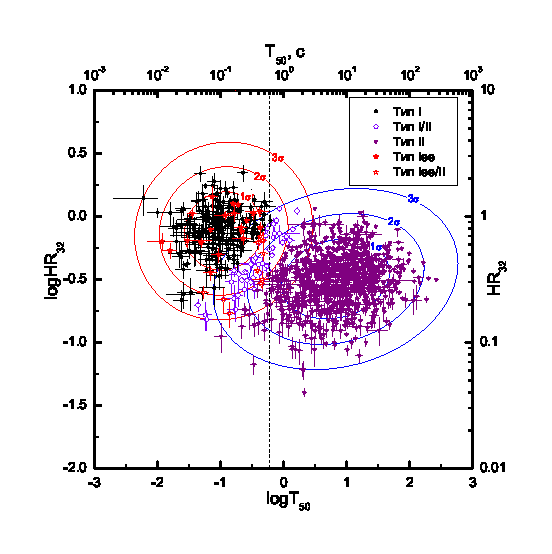
\includegraphics [width=0.6\textwidth,trim=0.5cm 0.2cm 0.5cm 0.5cm,clip] {gHRT50_Types_ru}
  \caption{Классификация 1143 ярких всплесков KW.
  Черные точки~--- Тип~I, круги~--- Тип~I/II, треугольники~--- Тип~II,
  звёздами показаны начальные импульсы всплесков типов Iee и Iee/II.
  Вертикальной пунктирной линией обозначена граница между длинными и короткими всплесками $T_{50}=0.5$~с.
  } 
  \label{img:HRvsT50Types}  
\end{figure}

Раздел~2.5 посвящен анализу спектральных задержек коротких всплесков. 
Показано, что всплески типа~I имеют незначительные спектральные задержки $\lesssim 25$~мс.
В разделе~2.6 показано, что для 121 всплеска KW предложенная классификация на основе 
соотношения жёсткость-длительность в гамма-диапазоне хорошо согласуется 
с их физической классификацией.
Сравнение распределений $\log T_{50}$--$\log \rmn{HR}_{32}$ в системе отсчёта наблюдателя 
и в космологической системе отсчёта показывает, что различие в жесткости и длительности
всплесков типов~I и~II становится менее значимым, но в целом сохраняется.

С учётом проведённого сравнения, события из набора 296 коротких всплесков 
были отнесены к физическим типам на основе полученной аппроксимации 
распределения $\log T_{50}$--$\log \rmn{HR}_{32}$. 
Определено, что $\sim 70$\% всплесков имеют Тип~I, 
$\sim 8$\% Тип~II и $\sim 12$\% имеют Тип~I/II. 
Доля коротких всплесков с EE составляет $\sim 10$\%.
Среди начальных импульсов всплесков, отнесённых на основе морфологии временной 
истории к коротким всплескам с EE, 21 (68\%) классифицированы как Тип~I (Iee), 3 как Тип~II 
и~7 как Тип~I/II (Iee/II).

\FloatBarrier

\underline{\textbf{Третья глава}} посвящена локализации выбранных коротких всплесков 
методом триангуляции с использованием межпланетной сети IPN~[A1], 
произведённой при активном участии соискателя. 

В разделах~3.1 и~3.2 приведено описание сети IPN и входящих в неё космических 
аппаратов и дана статистика наблюдений этими КА коротких всплесков KW. 
Раздел~3.3 посвящен описанию методики триангуляции. При детектировании GRB двумя КА 
было определено время распространения фронта излучения между КА методом кросс-корреляции 
измеренных кривых блеска. На основе определённого времени распространения
были построены локализации в форме колец на небесной сфере, см. рис.~\ref{img:Triangulation}.
Основной вклад в ошибку определения времени распространения для околоземных КА вносит
статистика отсчётов в кривой блеска, а для КА на межпланетных расстояниях~--- систематические 
ошибки временной привязки бортовых часов и временное разрешение детекторов.
В разделе~3.4 приведено подробное описание получения
колец для различных пар КА. Получено 517 триангуляционных колец.
В разделе~3.5 описано построение локализаций всплесков в виде пересечения колец. 
Иллюстрация локализации GRB методом триангуляции приведена на рис.~\ref{img:Triangulation}. 

\begin{figure} [h] 
  \center
  \includegraphics [width=0.6\textwidth] {annuli_ru.eps}
  \caption{Получение локализации GRB методом триангуляции [из~A2].
   Зная времена регистрации GRB на нескольких (в данном случае~--- трех) КА, 
   можно построить несколько триангуляционных колец, область пересечения которых содержит источник всплеска.} 
  \label{img:Triangulation}  
\end{figure}
\FloatBarrier
В итоге для 271 короткого гамма-всплеска KW получена наиболее полная локализационная информация. 
Из них для 17 точно локализованных всплесков триангуляционные кольца были получены для калибровки.
При участии соискателя, методом триангуляции также были получены локализации 146 гамма-всплесков,
зарегистрированных инструментом \textit{Fermi}-GBM за период с 12 июля 2008~г. по 11 июля 2010~г.
Было установлено, что IPN-триангуляции 
существенно улучшают локализации всплесков по сравнению с GBM, сокращая площадь 
области локализации всплеска в $\lesssim 180$~раз~[A2]. 
Раздел~3.6 посвящен 
локализации нескольких особо важных событий: кандидатов во внегалактические гигантские вспышки SGR 
и возможного слабого короткого всплеска от галактического SGR~1900$+$14.
В разделе~3.7 приведены результаты совместного поиска послесвечений гамма-всплесков IPN 
и системы телескопов Паломарской обсерватории iPTF. За период с 2013~г. по 2014~г. 
при помощи iPTF произведён поиск послесвечений в 35 локализациях гамма-всплесков, 
зарегистрированных \textit{Fermi}-GBM, для восьми из них было обнаружено послесвечение. 
В четырёх случаях поиск послесвечения был упрощён благодаря IPN локализации, 
полученных при активном участии соискателя~[A3]. 

\underline{\textbf{Четвертая глава}} посвящена поиску гигантских вспышек от SGR, 
расположенных в близких (до 30~Мпк) галактиках, выполненному соискателем.
В главе дана оценка чувствительности KW и IPN к гигантским вспышкам 
и приведены результаты поиска наложений локализаций всплесков на ближайшие галактики. 
В заключение приведена оценка частоты гигантских вспышек различной 
интенсивности~[A4].

В разделе~4.1 дан обзор наблюдательных проявлений SGR и описание ранее зарегистрированных 
кандидатов во внегалактические GF. В разделе~4.2 для KW и IPN оценено предельное 
расстояние детектирования GF со спектром и интенсивностью, аналогичными измеренным для GF от SGR~1806$-$20, 
которое составило $\sim 30$~Мпк. Показано, что менее интенсивные GF, сравнимые 
с GF от SGR~1900+14 и SGR~0526$-$66 могут быть зарегистрированы IPN в галактиках 
не далее $6$~Мпк.

В разделе~4.3 описан набор из 1896 близких ($\le 30$~Мпк) галактик, 
выбранных из каталога GWGC (Gravitational Wave Galaxy Catalogue,\citep{White2011CQGra}),
которые обеспечивают 90\% вспышек сверхновых внутри выбранного объёма.
Частота вспышек сверхновых была оценена исходя из абсолютной величины галактик 
в фильтре $B$ и их морфологического типа. 
В предположении, что количество SGR пропорционально частоте вспышек сверхновых, 
определены галактики, которые являются наиболее вероятными источниками GF. 
В дополнение к указанным в~\citep{Popov2006}, 
данный набор содержит PGC047885, IC~0342, NGC~6946, NGC~5457 и NGC~5194.
В разделе~4.4 дан анализ наложения 
локализаций коротких всплесков на галактики, отобранные из GWGC. Значимой 
корреляции локализаций всплесков и близкими галактиками не обнаружено. 
Были обнаружены только два всплеска, ранее ассоциированые 
с группой галактик M81/M82 (GRB~051103) и галактикой Андромеды (GRB~070201),
локализации которых имеют малую вероятность случайного наложения на эти галактики.
Дополнительный поиск всплесков из скопления Девы не выявил возможных кандидатов в GF.
В разделе~4.5 на основе предположения, что внутри объема $d \le 30$~Мпк наблюдалась 
только одна GF с энерговыделением $Q \gtrsim 10^{46}$~эрг в группе галактик M81/M82, 
получен верхний предел на частоту подобных GF, составляющий 
${(0.6\textrm{--}1.2)\times 10^{-4} Q_{46}^{-1.5}}$~год$^{-1}$~на~SGR.  
Данный предел предполагает появление порядка одной GF с таким энерговыделением 
за  характерное время активности SGR, составляющее $10^3\textrm{--}10^5$~лет. 
Этот предел вычислен на основе наибольшего на 2014~г.  
набора коротких всплесков и согласуется с ранее полученной в работе~\citep{Ofek_2007ApJ} оценкой. 
Для GF, сопоставимых по энерговыделению со вспышкой SGR~0526$-$66 5~марта~1979~г. ($Q \lesssim 10^{45}$~эрг), 
полученный верхний предел оказывается на порядок выше~--- $(0.9\textrm{--}1.7)\times 10^{-3}$~год$^{-1}$~SGR$^{-1}$,  
что может быть интерпретировано, как возможность наблюдать более одной GF за время жизни SGR.
Необходимо отметить, что хотя полученные верхние пределы являются достаточно жесткими, 
они содержат значительную неопределенность, связанную с
неопределённостью галактической частоты вспышек CCSN, расстояния до SGR~1806$-$20 и
предельного расстояния детектирования~IPN.

В \underline{\textbf{пятой главе}} приведена методика и результаты спектрального 
анализа 293 коротких гамма-всплесков, зарегистрированных~KW.

В разделах~5.1 и~5.2 описана методика спектрального анализа, приведены критерии 
выбора наиболее подходящей модели спектра
и методика вычисления интегральных ($S$) и пиковых ($F_\rmn{peak}$) энергетических потоков. 
Показано, что для 214 коротких всплесков KW возможен полноценный анализ многоканальных спектров. 
Для 79 более слабых всплесков были использованы трехканальные спектры, 
созданные на основе кривых блеска в каналах G1, G2 и G3. 
В разделе~5.3 приведены результаты спектрального анализа; обнаружено, 
что большинство многоканальных спектров наилучшим образом описываются моделью CPL,
модели с более жестким поведением в области высоких энергий требуются только для 4\% всплесков. 
Показатели степени $\alpha$ модели CPL распределены 
вокруг значения~$-0.5$. Распределение по $E_\rmn{p}$ для CPL имеет максимум около 500~кэВ 
и покрывает около двух порядков величины, максимальное $E_\rmn{p}$ для 
проанализированного набора составляет $\sim 3$~МэВ. 
Приведённые результаты показывают существенное отличие спектров коротких и длинных GRB, 
последние в основном описываются моделью BAND с показателями степени в области низких 
и высоких энергий $\alpha \sim -1$ и $\beta \sim -2.5$ и $E_\rmn{p}$ в диапазоне 50--1000~кэВ.
Указанное различие в параметрах спектров свидетельствует о различии в механизмах 
генерации излучения в длинных и коротких GRB.
Среди 214 всплесков с многоканальными спектрами обнаружено три события, 
для описания которых необходима дополнительная степенная 
спектральная компонента с фотонным индексом $\sim 2$. 
Эти всплески входят в 10\% наиболее интенсивных событий из набора. 
Интегральный спектр наиболее яркого всплеска GRB~031214 и его аппроксимация показаны 
на рис.~\ref{img:extra_PL_comp}.
Обнаруженная компонента, по-видимому, имеет ту же природу,
что и обнаруженная ранее в GRB~081024B~\citep{Abdo_2010ApJ_712_558A} и 
GRB~090510~\citep{Ackermann_2010ApJ_716_1178A} на основе данных обсерватории \textit{Fermi}.

\begin{figure}[h!] 
  \center
  \includegraphics [width=0.5\textwidth,trim=0.2cm 0.5cm 0.5cm 0.5cm,clip] {GRB20031214_T36655_EE_int_sp_ru}
  \caption{Аппроксимация интегрального спектра GRB~031214 суммой функций CPL+PL.
  Пунктирной линией показан вклад модели CPL, штриховой~--- PL.} 
  \label{img:extra_PL_comp}  
\end{figure}


В разделе~5.3 детально проанализировано 30 коротких всплесков с EE.
Для 21 события интенсивность EE оказалась достаточной 
для спектрального анализа. Показано, что спектры EE четырех всплесков типа~I могут 
быть описаны моделью CPL с достаточно высокой $E_\rmn{p} \sim 160$~кэВ--2.2~МэВ,
что, в сравнении с более ранними результатами~\citep{Bostanci_2013MNRAS,Kaneko_2015MNRAS}, 
существенно расширяет верхнюю границу наблюдаемой жесткости EE.  

Раздел~5.4 посвящен обсуждению полученных результатов.
В подразделе~5.4.1 произведено сравнение результатов спектрального анализа 
с параметрами выборок коротких всплесков из каталогов \textit{Fermi}-GBM~\citep{Gruber_2014ApJS} 
и \textit{CGRO}-BATSE~\citep{Goldstein_2013ApJS}. 
Показано, что в схожем диапазоне интегральных энергетических потоков доли всплесков, 
описываемые одинаковыми моделями, для KW и GBM согласуются. Обнаружено, что для BATSE 
дополнительным фактором, влияющим на увеличение доли расходящихся PL моделей, 
является относительно узкий спектральный диапазон.
Продемонстрировано хорошее согласие распределений параметров модели CPL 
по данным указанных экспериментов. 

\begin{figure}[h!]
    \begin{minipage}[h]{0.5\textwidth}
		\center{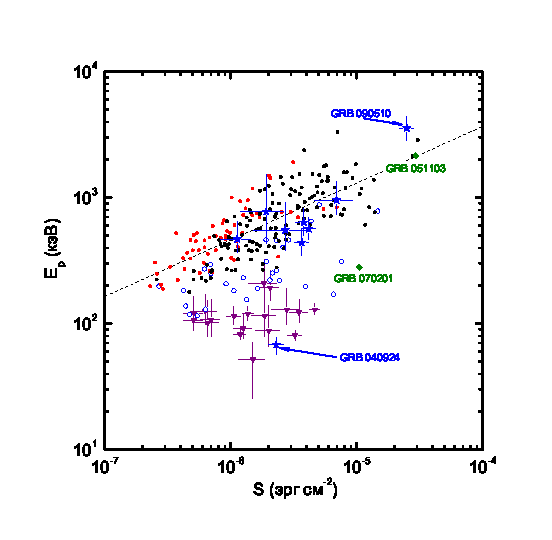
\includegraphics[width=1\textwidth,trim=0.5cm 0.4cm 0.5cm 0.5cm,clip]{gEpvsFl_ru.eps} \\ а)}
    \end{minipage}
    \hfill
    \begin{minipage}[h]{0.5\textwidth}
		\center{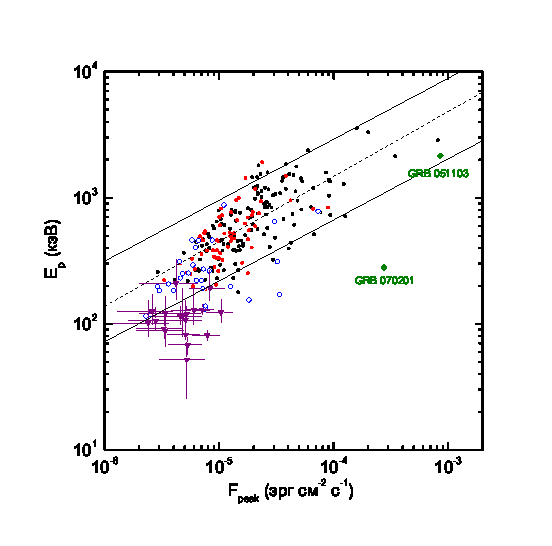
\includegraphics[width=1\textwidth,trim=0.5cm 0.4cm 0.5cm 0.5cm,clip]{gEpvsPF_ru.eps} \\ б)}
	\end{minipage}
    
\caption{\small
    Соотношения жёсткость-интенсивность (по результатам спектрального анализа с моделью CPL).
    На панели~(а) показано соотношение $E_\rmn{p}$ и $S$ для 139
    всплесков типа~I с многоканальными спектрами (чёрные точки); 
    65 всплесков типа~I с трёхканальными спектрами (красные точки); 
    29 всплесков типа~I/II (пустые точки), для обоих типов спектров;
    и для 19 всплесков типа~II (треугольники). Звёздами показаны 9 всплесков с известным красным смещением.
    На панели~(б) показано соотношение $E_\rmn{p}$ и $F_\rmn{peak}$ 
    для того же набора всплесков. Для всплесков типов~I и~I/II ошибки не показаны.
    Кандидаты в GF в близких галактиках обозначены ромбами. 
    Пунктирная линия соответствует степенной аппроксимации соотношений для всплесков типа~I,
    в обоих случаях индекс близок к $0.5$, сплошные линии~--- границы области, содержащей 90\% всплесков типа~I.
    % $E_\rmn{p}$--$S$ $\lambda = 0.45 \pm 0.16$
    % $E_\rmn{p}$--$F_\rmn{peak}$ $\lambda = 0.51 \pm 0.22$
    \label{img:EpvsFPandFL}}
\end{figure}

Подразделы~5.4.2--5.4.4 посвящены обсуждению результатов в контексте классификации всплесков на физические типы.
Исследование соотношений $E_\rmn{p}$ с $S$ и $F_\rmn{peak}$
(соотношения жёсткость-интенсивность; см. рис.~\ref{img:EpvsFPandFL}) показали, что:
(1)~предполагаемая GF в галактике M31 является явным выбросом в распределении $E_\rmn{p}$--$F_\rmn{peak}$, 
что подкрепляет свидетельства в пользу отличной от GRB природы этого события;
(2)~всплески типов I и~II занимают практически не пересекающиеся области на диаграмме $E_\rmn{p}$--$S$,
что подтверждает классификацию на основе параметров кривых блеска GRB.
Всплески типа~I образуют вытянутое распределение, которое в среднем подчиняется 
соотношению $E_\rmn{p} \propto S^{1/2}$. Всплески типа II образуют небольшую группу событий
с низкой $E_\rmn{p}$, которая представляет собой малую часть распределения длинных всплесков.
На плоскости $E_\rmn{p}$--$F_\rmn{peak}$ всплески Типа~II продлевают корреляцию 
жёсткость-интенсивность в область низких $E_\rmn{p}$ и малых $F_\rmn{peak}$.
Приведены доводы в пользу того, что всплески Типа~I подчиняются 
соотношению, аналогичному соотношению Амати~\citep{Amati_2002AandA} в космологической системе отсчёта.

Показано, что распределение по длительности начальных импульсов коротких всплесков 
типа~I с EE (Iee) согласуется с распределением для обычных коротких всплесков типа~I, 
о чем свидетельствует результат теста Колмогорова-Смирнова. 
Также было обнаружено, что начальные импульсы всплесков типа Iee в среднем 
жестче ($E_\rmn{p}$ в $\sim 1.5$ раза выше), чем всплески типа~I. 
Сопоставление распределений 
всплесков типов Iee и~I по $S$ и $F_\rmn{peak}$ выявило, что начальные импульсы 
всплесков с EE в среднем более интенсивные. 

Описанный в главе анализ выполнен лично соискателем.

\FloatBarrier
В \underline{\textbf{заключении}} приведены основные результаты работы, 
которые состоят в следующем:
\begin{enumerate}
 
\item Исследован временной дрейф параметров детекторов, долговременные вариации фона и оценен порог 
    срабатывания триггера KW, составляющий, в зависимости от временн\'{о}го масштаба 
    и параметров спектра всплеска, от $\sim 3\times 10^{-7}$~эрг~см$^{-2}$ до
    $\sim 1\times 10^{-6}$~эрг~см$^{-2}$. 
    
\item Для набора 1834 всплесков KW вычислены длительности $T_{50}$ и $T_{90}$, жесткости 
    и спектральные задержки. Показано, что распределения 
    всплесков по $T_{50}$ и $T_{90}$ хорошо аппроксимируются двумя логнормальными 
    распределениями. Обнаружено, что параметры аппроксимации распределения $T_{50}$ 
    более устойчивы к выбору порога поиска начала и конца всплеска, поэтому длительность 
    $T_{50}$ более предпочтительна для классификации всплесков. 
%    В качестве границы между длинными и короткими всплесками была выбрана точка 
%    пересечения логнормальных компонент для порога значимости $5\sigma$, $T_{50} = 0.6$~с. 
    Обнаружен 31 кандидат в короткие всплески с продлённым излучением.
    Выделен набор 296 коротких всплесков (с учётом кандидатов 
    в короткие гамма-всплески с продлённым излучением). 
      
    Аппроксимация распределения 1143 ярких всплесков KW на плоскости $\log T_{50}$--$\log \rmn{HR}_{32}$ 
    набором гауссовых компонент показала наличие 
    в данных KW двух классов всплесков: коротких/жестких и длинных/мягких. 
    Сравнение классификаций на физические типы~I и~II с классификацией на основе 
    длительности, жесткости и спектральной задержки подтвердило, что всплески Типа~I 
    относятся к коротким/жестким всплескам с малой спектральной задержкой, а всплески 
    Типа~II, в основном,~--- длинные мягкие с заметной спектральной задержкой. 
    
\item Получена наиболее полная локализационная информация для 271 короткого 
    гамма-всплеска KW. 
    Методика триангуляции была успешно применена для 
    локализации источников 146 гамма-всплесков, зарегистрированных \textit{Fermi}-GBM, и
    подтверждения оптических послесвечений, зарегистрированных системой телескопов 
    iPTF Паломарской обсерватории.
    
\item На основе оценки чувствительности эксперимента Конус-Винд и сети IPN получено 
    предельное расстояние регистрации GF от SGR, схожих с GF от SGR~1806$-$20, 
    равное $\sim 30$~Мпк. 
    Произведён поиск близких галактик в локализациях коротких гамма-всплесков KW. 
    Были обнаружены два всплеска, ранее 
    ассоциированы с группой галактик M81/M82 (GRB~051103) и галактикой Андромеды (GRB~070201),
    локализации которых имеют малую вероятность случайного наложения на эти галактики ($\sim 1$\%).
    Дополнительный поиск всплесков из скопления Девы не выявил возможных кандидатов в GF.
    
    Получен верхний предел на частоту GF с энерговыделением $Q \gtrsim 10^{46}$~эрг, равный
    $\sim 1 \times 10^{-4}$~год$^{-1}$~на~SGR, который предполагает 
    около одной GF с таким энерговыделением за время активности SGR ($10^3\textrm{--}10^5$~лет). 
    Этот предел был вычислен на основе наиболее широкого на 2014~г.  
    набора коротких всплесков и является более жестким, чем оценка ранее полученная в работе~\citep{Ofek_2007ApJ}.
    Для GF, сопоставимых по энерговыделению со вспышкой 5~марта~1979~г. ($Q \lesssim 10^{45}$~эрг), 
    полученный верхний предел на порядок выше~--- $\sim 1\times 10^{-3}$~год$^{-1}$~SGR$^{-1}$, 
    что может быть интерпретировано, как возможность наблюдать более одной подобной GF за время жизни SGR.
  
\item Выполнен спектральный анализ 293 коротких GRB, зарегистрированных KW. 
    Этот набор составляет $\sim 15$\% от полного числа всплесков, зарегистрированных 
    за первые 15~лет работы инструмента.
    Определены модели, наилучшим образом описывающие спектры всплесков и их параметры,
    на основе чего оценена наблюдаемая энергетика событий. 
    
    Среди 214 всплесков с многоканальными спектрами обнаружено три
    события, для описания которых необходима дополнительная степенная 
    спектральная компонента с фотонным индексом $\sim 2$. Эти всплески входят в 10\%
    наиболее интенсивных событий из набора. 
    Среди 21 короткого всплеска с EE, достаточно интенсивным
    для проведения спектрального анализа, обнаружено четыре события, у которых 
    начальный импульс классифицирован как Тип~I и спектр EE описывается моделью CPL 
    с относительно высокой $E_\rmn{p} \sim 160$~кэВ--2.2~МэВ. Полученный результат свидетельствует  
    в пользу наличия достаточно жесткого продлённого излучения у некоторых коротких гамма-всплесков. 
    
    Исследование соотношений $E_\rmn{p}$ с интегральным ($S$) и пиковым ($F_\rmn{peak}$) 
    энергетическим потоком (соотношения жёсткость-интенсивность) показали, что:
    (1)~Предполагаемая GF в галактике M31 является явным выбросом в распределении 
    $E_\rmn{p}$--$F_\rmn{peak}$,  что подкрепляет свидетельства в пользу отличной 
    от GRB природы этого события;
    (2)~Всплески типов I и~II занимают практически непересекающиеся области 
    на диаграмме $E_\rmn{p}$--$S$, что подтверждает их разную физическую классификацию, 
    предложенную соискателем на основе анализа кривых блеска и даёт возможность отделить события, 
    вызванные слиняем компактных объектов, от событий, связанных с коллапсом массивных звёзд.
  
\end{enumerate}


\subsection*{\Large Список работ, опубликованных по теме диссертации}
\setlist[description]{font=\normalfont}
\begin{description}
\item [A1.] Pal'shin\,V.\,D., Hurley\,K., Svinkin\,D.\,S. et al. Interplanetary Network Localizations of
Konus Short Gamma-Ray Bursts // Astrophys.~J.~Suppl.~--- 2013.~--- Vol.~207.~--- id~38;
\item [A2.] Hurley\,K., \dots\ , Svinkin\,D.\,S. et al. The Interplanetary Network Supplement to 
the Fermi GBM Catalog of Cosmic Gamma-Ray Bursts // Astrophys.~J.~Suppl.~--- 2013.~--- Vol.~207.~--- id~39;
\item [A3.] Singer\,L.\,P., \dots\ , Svinkin\,D.\,S. et al. The Needle in the 100 deg$^2$ Haystack: 
Uncovering Afterglows of Fermi GRBs with the Palomar Transient Factory // 
Astrophys.~J.~--- 2015.~--- Vol.~806.~--- P.~52;
\item [A4.] Svinkin\,D.\,S., Hurley\,K., Aptekar\,R.\,L., Golenetskii\,S.\,V., Frederiks\,D.\,D. \\ 
A search for giant flares from soft gamma-repeaters in nearby galaxies in the 
Konus-Wind short burst sample // Mon.~Not.~R.~Astron.~Soc.~--- 2015.~--- Vol.~447,~1.~--- P.~1028;
%\item D.~S. Svinkin, D.~D.~Frederiks, R.~L. Aptekar, et al.
%The second Konus-\textit{Wind} catalog of short gamma-ray bursts // submitted to ApJS;
%\item T.~N.~Ukwatta, K.~Hurley, J.~H.~MacGibbon, D.~S.~Svinkin, et al.
%Investigation of Primordial Black Hole Bursts using Interplanetary Network Gamma-ray Bursts // 
%arXiv:1512.01264, submitted to ApJ.

\end{description}

%\newpage
\renewcommand{\refname}{Литература, цитируемая в автореферате}

%\renewcommand{\refname}{\Large Публикации автора по теме диссертации}

\bibliography{../introduction,../part1,../part2,../part3,../part4,../part5} % Подключаем BibTeX-базы